%%%%%
%%
%% Sample document ``thesis.tex''
%%
%% Version: v0.2
%% Authors: Jean Martina, Rok Strnisa, Matej Urbas
%% Date: 30/07/2008
%%
%% Copyright (c) 2008-2011, Rok Strniša, Jean Martina, Matej Urbas
%% License: Simplified BSD License
%% License file: ./License
%% Original License URL: http://www.freebsd.org/copyright/freebsd-license.html
%%%%%

% Available documentclass options:
%
%   <all `report` document class options, e.g.: `a5paper`>
%   withindex   - enables the index. New index entries can be added through `\index{my entry}`
%   glossary    - enables the glossary.
%   techreport  - typesets the thesis in the technical report format.
%   firstyr     - formats the document as a first-year report.
%   times       - uses the `Times` font.
%   backrefs    - add back references in the Bibliography section
%
% For more info see `README.md`
\documentclass[withindex,glossary]{cam-thesis}

% Citations using numbers
\usepackage[numbers]{natbib}
\usepackage{todonotes}

%%%%%%%%%%%%%%%%%%%%%%%%%%%%%%%%%%%%%%%%%%%%%%%%%%%%%%%%%%%%%%%%%%%%%%%%%%%%%%%%
%% Thesis meta-information
%%

%% The title of the thesis:
\title{Towards Provenance as a First Class Construct of \\
Dependable Computing Systems}

% Alternate titles
% Provenance based trustworthiness assessment in computing systems

%% The full name of the author (e.g.: James Smith):
\author{Nikilesh Balakrishnan}

%% College affiliation:
\college{Churchill College}

%% College shield [optional]:
% \collegeshield{CollegeShields/Christs}
\collegeshield{CollegeShields/Churchill}
% \collegeshield{CollegeShields/Clare}
% \collegeshield{CollegeShields/ClareHall}
% \collegeshield{CollegeShields/CorpusChristi}
% \collegeshield{CollegeShields/Darwin}
% \collegeshield{CollegeShields/Downing}
% \collegeshield{CollegeShields/Emmanuel}
% \collegeshield{CollegeShields/Fitzwilliam}
% \collegeshield{CollegeShields/Girton}
% \collegeshield{CollegeShields/GonCaius}
% \collegeshield{CollegeShields/Homerton}
% \collegeshield{CollegeShields/HughesHall}
% \collegeshield{CollegeShields/Jesus}
% \collegeshield{CollegeShields/Kings}
% \collegeshield{CollegeShields/LucyCavendish}
% \collegeshield{CollegeShields/Magdalene}
% \collegeshield{CollegeShields/MurrayEdwards}
% \collegeshield{CollegeShields/Newnham}
% \collegeshield{CollegeShields/Pembroke}
% \collegeshield{CollegeShields/Peterhouse}
% \collegeshield{CollegeShields/Queens}
% \collegeshield{CollegeShields/Robinson}
% \collegeshield{CollegeShields/Selwyn}
% \collegeshield{CollegeShields/SidneySussex}
% \collegeshield{CollegeShields/StCatharines}
% \collegeshield{CollegeShields/StEdmunds}
% \collegeshield{CollegeShields/StJohns}
% \collegeshield{CollegeShields/Trinity}
% \collegeshield{CollegeShields/TrinityHall}
% \collegeshield{CollegeShields/Wolfson}
% \collegeshield{CollegeShields/FitzwilliamRed}

%% Submission date [optional]:
% \submissiondate{November, 2042}

%% You can redefine the submission notice [optional]:
% \submissionnotice{A badass thesis submitted on time for the Degree of PhD}

%% Declaration date:
\date{September, 2017}

%% PDF meta-info:
\subjectline{Computer Science}
\keywords{Provenance Dependable Assurance}



%%%%%%%%%%%%%%%%%%%%%%%%%%%%%%%%%%%%%%%%%%%%%%%%%%%%%%%%%%%%%%%%%%%%%%%%%%%%%%%%
%% Abstract:
%%
\abstract{%
\begin{itemize} 
\item Provenance capture in computing systems.
\item Use of provenance to reason about computations in the context of control flow and data flow.
\item We provide real implementations of systems that allows us to track computations in the context of scientific computing.
\item We also provide a prototype implementation of tracing data flow in the context of disk I/O, from the application to the device and back.
\end{itemize}
}



%%%%%%%%%%%%%%%%%%%%%%%%%%%%%%%%%%%%%%%%%%%%%%%%%%%%%%%%%%%%%%%%%%%%%%%%%%%%%%%%
%% Acknowledgements:
%%
\acknowledgements{%
  Add acknowledgements here ...
}



%%%%%%%%%%%%%%%%%%%%%%%%%%%%%%%%%%%%%%%%%%%%%%%%%%%%%%%%%%%%%%%%%%%%%%%%%%%%%%%%
%% Glossary [optional]:
%%
\newglossaryentry{HOL}{
    name=HOL,
    description={Higher-order logic}
}



%%%%%%%%%%%%%%%%%%%%%%%%%%%%%%%%%%%%%%%%%%%%%%%%%%%%%%%%%%%%%%%%%%%%%%%%%%%%%%%%
%% Contents:
%%
\begin{document}

%%%%%%%%%%%%%%%%%%%%%%%%%%%%%%%%%%%%%%%%%%%%%%%%%%%%%%%%%%%%%%%%%%%%%%%%%%%%%%%%
%% Title page, abstract, declaration etc.:
%% -    the title page (is automatically omitted in the technical report mode).
\frontmatter{}



%%%%%%%%%%%%%%%%%%%%%%%%%%%%%%%%%%%%%%%%%%%%%%%%%%%%%%%%%%%%%%%%%%%%%%%%%%%%%%%%
%% Thesis body:
%%
\chapter{The Need For Provenance}

\section{The Problem}
\begin{itemize}
\item Computing has become ubiquitous and pervasive.
\item Generation of large amounts of data.
\item More computing performed and decisions taken based on this data.
\item These results are then used in all aspects of society: Business, Science, Social and Government.
\item Business example from insurance, banking and e-commerce. Link real articles.
\item Examples from scientific computing, look at papers on cancer research etc. Look for other research that publishes results on data.
\item These computations are much more interleaved and used by each other. Take for example the 2008 debt crisis:
\item Financial products were created on top of other financial products and derivatives and new products where nobody understood
what they were actually representing. c.f. when people took on the product they did not understand the risk they were actually taking on.
\item Impact of these computations is huge. If the computation is wrong or inaccurate, it can have a huge impact on the structure of
society and/or have huge social, scientific, societal implications. Examples: e.g. Climate change controversy, Argentina Debt Crisis,
2008 Wall Street Crash etc.
\end{itemize}

\section{The Hypothesis}
\begin{itemize}
\item It is possible to build abstractions that allow people to track the inputs, operations and outputs of a computation
(provenance of a computation) so that you can reason about it from both a time and space perspective as you use the data
produced by the computation.
\item Having this support will allow us to mitigate the trust issues that arise from non-ascertainable computations.
\end{itemize}


\section{Thesis outline}
\begin{itemize}
\item In this thesis I explore the fundamental primitives required to build systems that offer provenance as a first-class construct
of systems.
\item To this end I focus on two systems:
(i) OPUS: A system for adding control-flow provenance to scientific computational pipelines.
(ii) NORAD: Non-repudiable assertions for disk I/O. NORAD is a system for asserting about data-flow in a computational system.
\item For each of these systems I provide real-world engineering systems and outline the design-space, implementation and use-cases for these systems.
\item I conclude by offering a look into further directions.
\end{itemize}

\section{Contributions}
The contributions of this thesis are thus:
\begin{itemize}
\item Design and implementation of a provenance system called OPUS, for scientific workloads.
\item Tools and applications that utilise this system to show its utility in the context of scientific computation.
\item A performance characterisation of the system compared to existing systems.
\item A prototype system, NORAD for asserting the data provenance captured by provenance systems.
\item A characterisation of NORAD's performance and use-cases showing its utility.
\end{itemize}

\chapter{A Background into Provenance}
This chapter presents the background literature in the area of provenance.
\begin{itemize}
\item What is provenance and what is the use of provenance? A systematic capture of meta-data that describes the where, when and how of data and computations.
\item Meta-data is typically a graph that describes relationships between various elements or entities in a system that contributed to a piece of data produced by the system.
\item How is it captured?
\item Brief introduction into the various capture approaches used, system, workflow, database, etc. Our interest is in providing this support at the system level.
\item Therefore we focus on those mechanisms that capture provenance at the system call, filesystem and OS layers.
\item Introduce the concept of granularity of capture, the layer at which the capture happens and what the provenance describes at each layer of abstraction.
\item How provenance can be queried and used?
\item What about the security of the provenance itself? Current state-of-art in provenance security is the SPROV work that ensures the integrity and authenticity if provenance records once its captured.
\item What about provenance that was circumvented or falsified at the point of capture?
\item Cite the Primer on Provenance paper.
\end{itemize}

\chapter{OPUS: Provenance Support for Scientific Workloads}
The work described in this chapter is a joint contribution with Thomas Bytheway. My primary contribution in this body of work is as follows:

\begin{itemize}
\item Equal intellectual contribution with Thomas Bytheway in the system design of OPUS.
\item Participated and contributed in the discussions on PVM, especially in modelling corner cases using PVM.
\item Implemented most of the interposition mechanism in the OPUS front-end.
\item Re-implemented parts of the OPUS backend to work with a graph database store, Neo4J.
\end{itemize}

\section{Introduction}
In ~\ref{ch:two} we have seen previous approaches for provenance capture, query and some real-world use-cases for provenance. In this chapter we attempt to outline the shortcomings of existing provenance systems, detailing the problems as the motivation for the design and implementation of OPUS, a user-space provenance capture, analysis and query tool for scientific computing. We show that it is possible to build tools and applications that can use this provenance captured to aid in tracking, archiving and debugging of multi-step ad hoc scientific computations.

\section{Motivation}
Today most physical sciences are computation based.
At its core, scientific computations involve the development of models and simulations to understand the natural world. 
These models and simulations are typically composed of multiple computational steps where data is input and output within each step, forming an experiment pipeline wherein data output in a step is used as input in the next step.
Once a result is obtained and interpreted, confidence in the result is obtained by analysing, repeating and reproducing the experiment independently.
In order to do this scientists have traditionally used manual and ad hoc techniques to record the data inputs and contexts (parameters, configuration, dependencies etc.) used in the computations to produce the result.
This manual process is however prone to errors and often not complete, resulting in experiments not being reproducible ~\cite{non-rep, nature}. 
Provenance systems ~\cite{PASS, BURRITO, StoyBook} in the past have attempted to automate this effort and ease the process of reproducibility by automatically tracking data and computation.
However, these systems have lacked adoption in the real-world and have merely resulted in being research or experimental prototypes.
This is primarily because these systems are not widely available or easily deployable in practice.
Most of these systems require changes to the existing workflows, require modification to the underlying OS or require the use of specialised systems.
Our goal is to design and implement a lightweight, general purpose provenance system that has a minimum barrier to entry, especially in the context of scientific computing.
To this end, we have designed OPUS, a provenance system that is designed to work entirely in user-space and is based on several key design constraints discussed in the next section ~\ref{sec:constraints}.

\section{A unique constraint space}
OPUS draws inspiration from previous approaches in building general purpose provenance systems but addresses several of their shortcomings outlined in ~\ref{sec:opusmotiv}. The design of OPUS is based on the following requiements:

\begin{itemize}

\item \textbf{Non-intrusiveness:}
It is our observation that most computational scientists seldom have \texttt{root} or system level access to install and update software. Therefore it is important for a general purpose system to be as non-intrusive as possible i.e. the system should not require changes to the underlying OS or the use of bespoke kernel modules to capture provenance. Therefore a major design principle for OPUS is that it must work entirely in user-space. An added advantage of designing OPUS to work in user-space is that it becomes easier to ensure that in a shared system, users of OPUS do not affect other users in the system.

\item \textbf{Ease of installation:}
In addition to being non-intrusive a general purpose provenance system must be easy to install. The installation must be self-contained, having no external dependencies and requiring minimal configuration changes. This ensures that the barrier to adoption of such systems by users such as scientists is as low as possible.

\item \textbf{Seamlessness:}
Scientific computing across disciplines are diverse in terms of the workflow used, therefore a general purpose provenance system should not require the users to modify their existing workflow in order to use the system. OPUS should therefore be designed to drop into a user's environment and seamlessly integrate with existing workflows and capture provenance.

\item \textbf{Low overheads:} 
Scientific applications are typically executed multiple times and each run can perform multiple iterations until the computation converges to a specific expected result. This execution could therefore take anywhere from seconds to minutes to hours depending on the complexity of the computation performed. Therefore it is important that a provenance system like OPUS impose minimal overheads on the application run time. Similarly, the application could be executing in memory and storage constrained environments, therefore keeping the spatial overheads low is also a useful property to consider while designing the system.

\item \textbf{Completeness:} 
Existing systems record only a subset of operations applications perform on files and processes. This restricts the range of provenance queries that one can implement. To support a richer set of queries OPUS should be designed to capture all file and process relatede operations. Also, merely capturing file and process interactions ignores the execution context (library versions used, command line parameters used, environment variables etc.) in which these operations were done. Therefore the mechanism OPUS uses should capture the surrounding execution context as well. 

\item \textbf{Reasoning about provenance:} \todo{This needs a rewrite}
The ultimate goal of capturing provenance is to use it to reason about application execution and data used or produced. However, provenance is itself represented and stored as data, therefore we require a structured mechanism to reason about provenance data as it is recorded and stored. Existing systems are either rigid or use ad-hoc approaches to record and store provenance. In order for provenance to be useful and effective, we require a more formal approach to reason about the provenance data itself. In section ~\ref{sec:pvm} we discuss PVM, a semi-formal model for representing provenance.

\end{itemize}

\section{Design Decisions} \todo{Write the section on design and implementation of OPUS here}
The design of OPUS is guided by the constraints outlined in ~\ref{sec:constspace}.
The initial design is intended for on-host provenance capture, analysis and query.
In this section we discuss our approach and some of the decisions involved in designing OPUS.


\subsection{Provenance Capture}
One of the main components in the design of OPUS is the provenance capture component.
In the context of scientific computing, our requirement for OPUS is to employ a seamless, non-intrusive, always-on and lightweight method for provenance capture.
To build such a system we explore several existing mechanisms to capture provenance.
A key observation here is that most of these mechanims have conventionally been used in tracing and debugging applications.
Since the data captured by these techniques overlaps to a considerable amount with the data required for provenance we can leverage these mechanisms to build provenance systems.

\paragraph{FUSE} is a framework that allows non-privileged users to implement a custom filesystem in user-space. FUSE consists of (i) a kernel module which registers a filesystem with the kernel's virtual file system (VFS) and (ii) a user-level daemon that either implements the entire filesystem functionality or acts as a pass-through layer to a kernel filesystem. A proof-of-concept system ~\cite{StoryBook} has shown that it is possible to use this framework to capture I/O activities of applications and can be done without any modification to the application or existing workflows as perceived by the user. Therefore for OPUS, FUSE is a viable option for provenance capture. However, the use of FUSE for provenance capture has several limitations:
(i) FUSE requires root permissions to install and configure.
(ii) With certain workloads FUSE can impose a significant overhead on application I/O ~\cite{StoryBook}.
(iii) FUSE only intercepts I/O activities, other crucial process level operations required to build more richer provenance is not visible to FUSE.

\paragraph{PTrace} is a process tracing functionality supported on most Unix-like OSes. 
PTrace allows a tracer process to trace the execution of a target process.
When an event of interest (for example system calls) is executed by the target, the underlying OS stops the execution of the traget and switches control to the tracer process.
The tracer process can then examine the register and memory state of the target process.
This is the core mechanisms used to implement debuggers.
This can be a useful technique to capture provenance as well since it provides complete visibility into the target program's execution.
The primary advantage of using PTrace for provenance capture is that is does not require root permissions unless the target process is executing as root.
However, PTrace imposes a high temporal overhead (~30\%) on the process being traced since the mechanism requires multiple context switches for each event being traced.
This makes PTrace impractical for use in an always-on, system-wide provenance capture system.

% TODO: Make this consistent with other paragraphs
\paragraph{Kernel-level Tracing:}
Over the years systems developers have recognised the need for a flexible tracing infrastructure for both the kernel and user-space applications.
A number of mechanisms and tools ~\cite{DTrace, SystemTap, Uprobes, LXCModules} have been created to support this requirement.
The core idea with these mechanisms is to provide support in the kernel to trace application activity, typically by monitoring the interaction of the application with the OS.
The key benefits of kernel-level tracing mechanisms are that it is completely seamleass to applications, executes at a higher privilege level and therefore potentially secure from user-space attacks.
A user will require \texttt{root} permissions to enable or configure these tracing mechanisms.
However, the main limitation of using such an approach for provenance capture is that most of these mechanisms have been introduced fairly recently and they may not be supported in older kernel versions.
Given that our requirement is to support scientific workloads our initial decision is to not use such techniques for provenance capture.


\paragraph{Binary Rewriting} is the process of transforming an application binary by modifying individual instructions to implement a specific functionality while still retaining the semantics of the original application. 
Binary rewriting can happen either (i) statically, where the application binary is disassembled and the instructions are modified or (ii) dynamically, where the instruction stream is modified at runtime using just-in-time compilation. 
Provenance capture can be implemented using such mechanisms wherein specific instructions (for e.g. syscall instruction) executed by the application are intercepted and captured.
Manually implementing this correctly and in a generic manner is a difficult exercise, however, there are a number of tools and frameworks ~\cite{PIN, DynInst} that can significantly ease this process.
Given that this mechanism can be implemented entirely in user-space it can be considered a viable method for provenance capture for a system like OPUS.
However, for the initial design our goal is to use a quicker approach for prototyping the system, therefore binary rewriting may not be the ideal choice to implement the capture component.

\paragraph{LD\_PRELOAD:} is a feature provided by the runtime linker that enables overriding of symbols in libraries linked by programs at load time. In order to override the symbols, a new library with definitions for the symbols to be overridden must be implemented and the environment variable LD\_PRELOAD set to this library path. In the context of provenance capture we can use this mechanism to interpose calls made by applications to the standard C library. Given that the standard C library is a wrapper over the system call interface, this becomes a viable method for capturing provenance at system call granularity.
The primary advantages of the LD\_PRELOAD mechanism is that (i) it imposes a much lower overhead when compared to other user-space system call interception mechanisms and (ii) it is easier to implement and prototype since there is no special API or interface required to implement it.
However, LD\_PRELOAD assumes that applications link with the standard C library dynamically and that system calls are always invoked by application via the C library.
For a system that captures provenance in the context of scientific computing it is reasonable to assume that most programs dynamically link with and interface with the OS using the C library. Given that this mechanism satisfies a majority of the requirements for a lightweight, userspace provenance capture system, our decision for the first version of OPUS is to employ library interposition as a method for provenance capture.


\subsection{Provenance Analysis} % TODO: Refine this further
The raw provenance stream consisting of system call event data from executing programs should be converted to a meaningful representation that describes the provenance of processes, files, sockets etc.
In previous general purpose provenance systems ~\cite{PASS, PASSv2} this has been represented as a directed acyclic graph (DAG) where the nodes represent entities such as processes and files while the edges describe the interation between these entities as shown in figure xxx.% TODO: Show a simple DAG of processes and files.
OPUS uses a similar approach and collects event streams from processes executing on the machine and converts it into a provenance graph.
However, unlike previous systems, OPUS uses a semi-formal model, PVM (Provenance Versioning Model) to map and model the undelying system semantics.
PVM formalises the process by which entities in the graph are updated and allows us to reason about changes to these entities.
PVM is discussed in detail in section~\ref{sec:PVM}

\paragraph{On-host or Off-host analysis?}
The provenance analysis component of OPUS can run on the same host where system call events are captured or off-host, on a dedicated server.
Our initial design assumes that all event streams from a single host will be handled by an analyser instance dedicated for that host.
However, given the context of scientific computing our goal is to make OPUS easy to adopt and minimise the barrier to entry, to this end our initial version of OPUS will run the analysis component on the same host where capture is performed.

\paragraph{Event Ordering:}
Maintaining a correct view of order of events in the system is important for provenance systems since small changes in the order of events can produce significant semantic changes to the graph being generated.
For example, consider two events in the system, event \texttt{E1} where a process \texttt{P1} opens a file \texttt{F} to write to it and another event \texttt{E2} wherein a process \texttt{P2} unlinks \texttt{F}.
In such situations, processing events in the correct order is crucial in order to reflect the actual side-effects these operations have on the underlying system.

A naive approach to implement ordering is to use the system clock to timestamp events.
However, the system clock for a given machine is not guaranteed to be sane over any period due to NTP updates or users manually changing the system time.
Therefore using the system clock is not a reliable method to order events.
A more reliable approach is to use the machine's hardware monotonic clock as it provides the guarantee of a consistent increasing time value over any single run of a given machine.
With the initial version of OPUS we favour this approach, especially since we plan to run a dedicated instance of OPUS on-host.

\subsection{Provenance Storage}
Once the raw system call events are received by the OPUS backend and transformed into provenance using PVM rules, it must be persisted in a suitable data store.
As part of the design we consider primarly three types of data stores:

\paragraph{Relational:} 
Relational databases have been around for decades and are the database of choice for many data-intensive storage and retrieval applications.
Most relational databases support SQL as the standard language for queries and this makes transitioning between various implementations of relational databases much easier.
However, given the graph structure of our provenance data, expressing traversal queries for relational data can result in exceedingly complex queries.
At the time of designing OPUS there was a lack of support for hierarchical queries in SQL therefore relational databases was not first choice for our data store.
Today, there is support for Common Table Expressions (CTEs) which allow us to effeciently express complex traversal queries in relational databases.
For the initial implementation of OPUS we need to ensure that the data is easily storable and retrievable for the purposes of tracking scientific data and computation, therefore relational databases may not be the best fit for our needs.

\paragraph{Key-Value:}
Key-Value databases have gained popularity in recent times mainly because they are schemaless and simple to use. They and desgined for storing, retrieving and managing associative arrays.
KV stores are avialable for a range of applications from heavy weight distributed systems to single node systems running as an embedded database instance within applications.
Previous general purpose provenance systems such as PASS have shown that it is possible to use key-value stores ~\cite{BerkleyDB} for the storage and retrieval of provenance.
During the design and implementation of OPUS we've explored the use of LevelDB an embedded key-value store by modelling nodes and edges in the provenance graph to fit the key-value paradigm.
We've observed that although key-value stores are simple to integrate with and use, they have several downsides while modelling provenance graph structured data:
(i) The implementation of features like node and edge types in key-value stores requires partitioning of the key space to encode type information.
(ii) Indexes on node and edge properties have to be manually implemented as key-value stores inherently do not support indexes.
(iii) They do not provide support for an expressive query language such as SQL. Instead, graph traversal queries must be implemented manually at the application layer. This results in an increased number of round-trips to the database and back, leading to a reduction in performance.

Given these shortcomings, our conclusion is that key-value stores are not the best fit for the first phase of OPUS.

\paragraph{Graph:} 
Graph databases can represent our provenance object and relationships more naturally and effectively.
Most graph databases also allow for powerful querying capabilities either via a query language such as Cypher ~\cite{Cypher}  or a traversal API ~\cite{Gremlin}.
For the initial design and implementation of OPUS our requirement is to use a lightweight and easily administerable graph database, while also providing the possibility of scaling the database in future if required.
Given this constraint our decision is to use an embedded Neo4J database to run as part of the OPUS backend (Provenance Analyser) to persist provenance data.
Neo4J also provides the option to scale out to running a dedicated server instance or to cluster several instances if necessary.
This augurs well for our future requirements as well.

% -----------------------------------------------------------------------------

%Databases to consider?
%
%Target is scientific computing environment. Need a lightweight d/b that requires little or no maintenance.
%Our focus therefore was to use an embedded DB. Single host, tightly coupled, little ongoing maintenance etc.
%
%Relational, Graph, Key-Value?
%
%Relational: Been around for a long time. Scalable to large datasets. Most DBs support SQL based querying. 
%May not be the most efficient way to represent graph structured data.
%SQL languge support at the time of designing OPUS lacked semantics for graph type queries.
%Today SQL has support for CTEs with most relational dbs.
%
%Graph Databases: Seeing a surge in graph dbs. Most are however designed for distributed storage. Also quite heavy weight and over-engineered.
%We need something more simpler.
%Our initial plan is to build this prototype quickly and reevaluate the storage layer in the next phase.
%
%KV-store: Simple operations get and put. No schema required. Very simple and lightweight. Plethora of implementations from in-memory, embedded persistent to distributed.
%All pretty much supporting the same operations.
%Previous systems such as PASS have also used KV stores to for persistence of provenance. It has been shown to work.
%For the initial implementation we experimented with a KV-store, LevelDB as it is embedded and has relatively good performance numbers compared to other state of art embedded dbs ~\cite{leveldbBench}. 
%However, this was not tenable since a query language is not supported. Most of the traversal queries need to be performed manually resulting in a lot of round-trips betwen the analyser and the d/b engine, leading to a lack of performance.

% -----------------------------------------------------------------------------

\section{System Design}
In this section we describe the system architecture of OPUS and the high level implementation details of each component of the system.

\begin{figure}[t!]
  \centering
    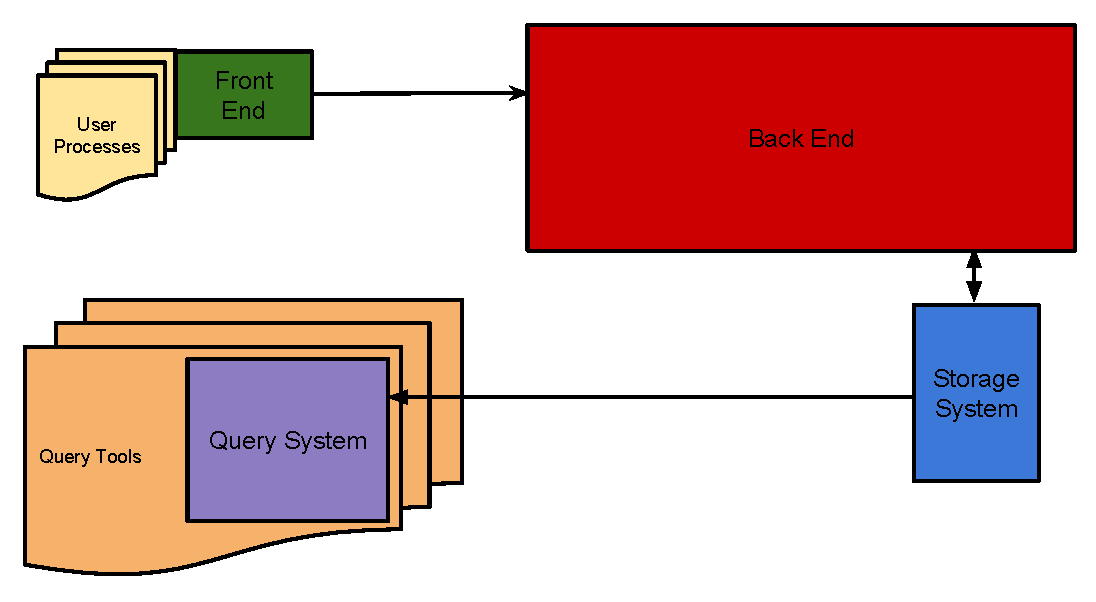
\includegraphics[width=1.0\columnwidth]{BroadProvDesign}
  \caption{OPUS: High Level Design}
  \label{fig:opushld}
\end{figure}

As shown in figure ~\ref{fig:opushld} the system consists of four main components:
\begin{itemize}
\item A frontend that captures raw event data from user activities.
\item A backend that analyses the raw event data and transforms them into a provenance graph.
\item A storage system that persists provenance objects and their relationships.
\item A query API that allows users to retrieve the provenance of their data and computations.
\end{itemize} 

The design of the system is such that multiple frontend instances can run simultaneously and transmit their event stream to the backend for analysis and storage.
%The initial implementation of the system for use in the context of scientific computing will use libc interposition for the events stream capture.
%Other producers using a different method for capturing event streams, for example kernel level instrumentation can easily be plugged into the system if necessary.
The backend for the initial phase will comprise of a single analyser instance running on-host that converts raw event streams into provenance.
However, the design can be extended to add multiple analyser instances to load balance or handle events from multiple hosts.
The storage system is also pluggable and the design allows this component to be changed in future releases.

\subsection{System Assumptions}
The current implementation of OPUS targets the x86 and x86\_64 processor architectures.
However, the design of OPUS itself is not machine or hardware dependent and can be easily ported to work on other architectures.
We assume that most applications, specifically scientific applications interact with the OS via libc and that that direct invocation of system calls are absent or rare.
Finally, we also assume that most scientific applications dynamically link with libc as the intersposition mechanism relies on the runtime linker.

\subsection{Module Level Desgin}

\begin{figure}[t!]
  \centering
    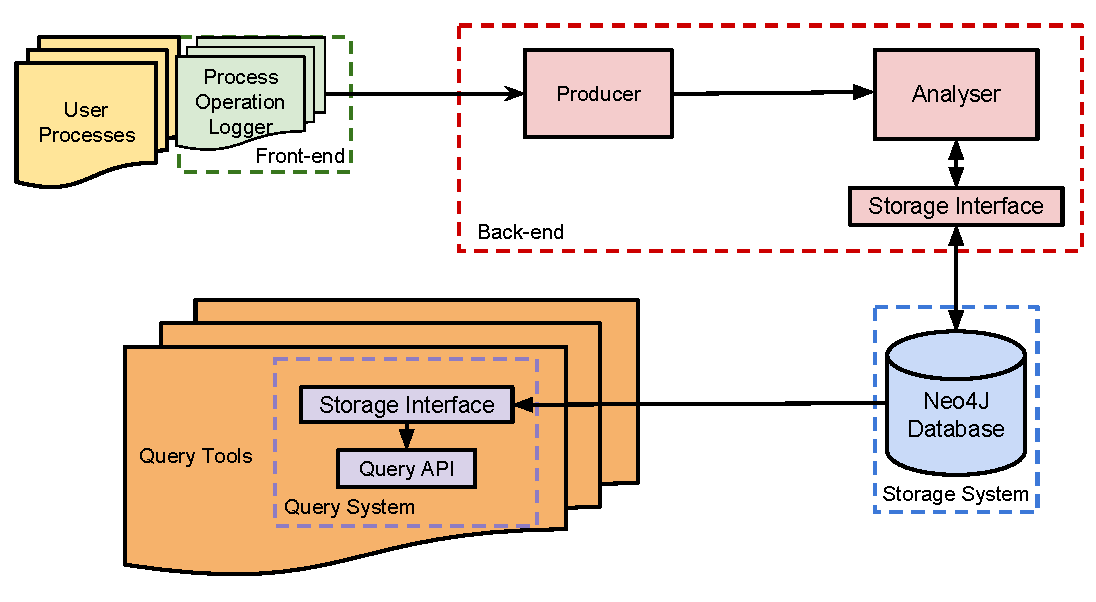
\includegraphics[width=1.0\columnwidth]{ProvDesign}
  \caption{OPUS: Module level design}
  \label{fig:opuslld}
\end{figure}

As shown in ~\ref{fig:opuslld} the primary modules in OPUS consists of a interposition module, connection manager, provenance analyser, storage interface and a graph database.
We now describe implementation details for each of these modules:

\subsubsection{Interposition Module}
The interposition module is a shared library implemented in C++.
This library is loaded transparently on program startup by setting the LD\_PRELOAD environment variable to point to the interposition library path.
Once this is done, when the program binary is loaded into memory, the runtime linker overrides the symbol table with the symbols defined as part of the interposition library.
When the program invokes a function call with an overridden symbol, the call first transfers to the interposition function which then calls the actual implementation. 
This is shown in \ref{fig:iposeexample} where a program calls an overridden symbol for the \texttt{open} libC function, resulting in the interposed function for \texttt{open} being executed first before calling the underlying libC implementation of \texttt{open}.
OPUS uses the interposition function to capture raw provenance information such as arguments passed to the function, its return value and program context.
The program context uniquely identifies the program/thread instance along with a monotonic timestamp to indicate the start and end of the event etc.
This raw provenance data is then packaged using Google's protocol buffers and sent to the backend for further processing.

Conceptually, implementing an interposition library is relatively straightforward.
It involves defining relevant functions with the same symbols as the target library functions, capturing the required arguments, calling the original function implementation and storing the return value.
However, in practice there are several technical challenges that arise while implementing a practically usable interposition library for capturing provenance:

\begin{enumerate}
\item \texttt{Growing Interposition Requirements:} Unlike system call interception, library call interposition requires implementing wrapper functions for all visible symbols. To understand this consider the \texttt{read} system call in the libC API. Figure ~\ref{fig:callchain} shows a sub-graph containing various paths through which the \texttt{read} function can be reached from withing the libC call graph. 
Here, merely interposing the final \texttt{read} function (also called stem function) does not result in interposing all other variants of the function since the \texttt{read} symbol is declared PROTECTED. The PROTECTED attribute ensures that internal calls in libC are computed at compile time instead of resolving at run-time.
This results in an explosion in interposition requirements since the a typical libC library implementation has over 1500 symbols that can be overridden. 

Manually implementing interposition for for these functions is cumbersome, not only due to the number of functions but also due to the different set of arguments and return values for each of these functions. The OPUS frontend deals with this problem by using code generating based on templating for most of the interposed functions. The details of how this is implemented is desribed in our paper ~\cite{OPUSLessons}.

\item \texttt{Maintaining Semantic Equivalence with Posix:} Another major issue with interposition is that when certain functions are interposed they can cause a change to application semantics. For OPUS, this is observed in the case of two functions, \texttt{vfork} and \texttt{signal}. Interposing these functions breaks the semantics expected by the application for different reasons. Both these cases are discussed in detail in our paper ~\cite{OPUSLessons} and how OPUS addresses these problems.

\end{enumerate}

\subsubsection{Connection Manager}
The OPUS backend implements a connection manager module that receives raw provenance data from applications being interposed.
The connection manager can receive this data via TCP or via UDS sockets and therefore is flexible to run on the same machine or on a remote machine.
The connection manager accepts data streams as protocol buffer messages from each frontend instance and adds these message to an internal priority queue that it shares with the Provenance analyser module.
A priority queue is used to ensure that the messages are sorted by their timestamp before being processed.

\subsubsection{Provenance Analyser}
The provenance analyser is the heart of the OPUS backend.
The analyser tranforms raw libC or system call events captured in the OPUS frontend into meaningful provenance graphs.
The analyser maintains a mapping of raw events to its corresponding action on the provenance graph based on PVM semantics.
The semantics of PVM is discussed in detail in section ~\ref{sec:pvm}.

Once the PVM definition for a given action is obtained, the provenance analyser can take decisions involving versioning provenance objects, linking provenance objects based on the type of operation performed and updating relevant I/O information in the provenance system.
This is illustrated with an example given below.

These actions typically involve decision regarding versioning of provenance objects, linking provenance objects based on type of operation performed and updating relevant event information in the graph.
As the graph is constructed, it is persisted via the storage interface described next.

\subsubsection{Storage Interface}
The storage interface provides an abstract interface for the analyser to store or retrieve provenance objects.
This abstraction allows the OPUS backend to use a wide variety of data stores for storing provenance.
For the initial implementation of OPUS, levelDB, a key-value store was considered as the storage backend, however, due to the lack of querying capabilities offered by key-value stores the current implementation uses the Neo4J graph database.

\subsubsection{Query API}
The query API provides a wide variety of functions to retrieve provenance data from the underlying data store.
The query API is implemented as a module that can be imported by any query tool.

% TODO: from here..
\section{Reasoning About Provenance}
Provenance systems are designed to store the history or lineage of digital entities such as files, sockets, pipes, processes etc.
Entities are typically modelled as objects and versioned in response to modifications by operations that change their state.
Versioning can thereby be defined as the recording of object state at semantically relevant epochs.
The goal of versioning is to relate object state with distinct, specific time epochs in the object timeline.
Typically, versions are chained, i.e. a version of an object links back to its previous representation.
It also gives us a weak sense of ordering of events.
Therefore versioning assists in reasioning about object state and is useful in optimising provenance queries.

\subsection{Types of Versioning Models}
Traditionally systems that capture and store provenance have relied on two well established versioning model.
\texttt{Version-on-Write} and \texttt{Open-to-Close}.

\paragraph{Version-on-Write:}
Version-on-write is perhaphs the simplest versioning model where a new object version is created on every action that mutates an entity.
It is also the easiest model to implement and reason about since each version of an object is associated with a distinct causal event in an entity's timline.
However, creating a new object version for each write can potentially result in a large number of versions and cause in a \texttt{provenance explosion}.
This can result in high spatial overheads for the system and make queries expensive since traversals through the resulting graph can be very long.
Also, a scheme like version-on-write does not explicitly specify how to model operations that do not mutate an entity's state, for e.g. a \texttt{read} operation.
Thefore such a model may not be suitable for a complete general purpose provenance system such as OPUS.

\paragraph{Open-to-Close:}
In the open-to-close approach versions are defined relative to \texttt{open} and \texttt{close} events.
A new version of an object is typically created on the first update to a block after an \texttt{open} and all operations on that entity are then associated to that new object version until the last \texttt{close} operation is invoked.

The main advantage of this versioning scheme is that we have clear start and end points for periods of manipulation of objects.
This also results in a concise graph representation.
However, the primary disadvantages of \texttt{open-to-close} is,
(i) Operations that do not invoke the \texttt{open} and \texttt{close} opeartions explicitly must be adapted to use these semantics, for e.g. the \texttt{stat} operation.
(ii) It is not possible to version on operations that cannot be implicitely or explicitely represented as an \texttt{open} and \texttt{close}.

A system like OPUS that is being designed for use in the real-world must be able to model and reason about provenance for a diverse set of entities each supporting their own set of operations and semantics. Therefore a rigid scheme like \texttt{open-to-close} is insufficient to meet those requirements.

\subsection{Definable Versioning Semantics}
Both \texttt{version-on-write} and \texttt{open-to-close} versioning models have the following drawbacks:
\begin{itemize}
\item Their provenance versioning semantics is implicitly based on the underlying system semantics on which they are implemented.
\item They are defined with focus on recording rather than logically reasoning about changes to objects.
\item They have been defined based on the constraint that versioning will only be carried out on object mutation or dereference.
\end{itemize}

We need a more abstract, expressive and flexible versioning semantics that can be defined independently and orthoganally to the underlying system versioning semantics.
By providing an abstarct and system decoupled versioning semantics we get the following properties:
\begin{itemize}
\item Extensibility - The versioning scheme is extensible to model a variety of system semantics, for example file access, network access, memory access etc.
\item Reasoning - We can reason about the versioning semantics itself, for example to reason about completeness or consistency of the semantic.
\end{itemize}

In section ~\ref{subsec:pvm} we describe PVM, a versioning model that offers these properties.

\subsection{PVM: Provenance Versioning Model}
PVM is an elementary model designed to enable the ratification of and reasoning about update semantics in provenance systems.
In essence PVM enables us to:
(i) formalise the concept of tracking and recording changes in system entities (i.e. versioning) and
(ii) formalise the versioning side-effects of concurrent updates to system entities.

\subsubsection{PVM Definitions}
In this section we will discuss some of the terminologies and operations used in PVM.

\paragraph{Object}
In PVM the basic unit of modelling is an \texttt{object}.
Objects are abstractions that group associated data and metadata in a logically addressable unit.
Objects typically represent system entities such as files, sockets, pipes etc.
Objects are uniquely addressable and accessible using an identifier, for example file path, IP address and port tuple etc.

\paragraph{Processes} are abstractions for entities that access or modify objects as a side-effect of execution.
These side-effects are operations that \texttt{processes} perform to \texttt{mutate} data or meta-data of an underlying entity (e.g. a file in unix) represented by its \texttt{object} in PVM.
An example of a \texttt{process} entity in PVM is a thread of execution in a UNIX like system.
It is also assumed that operations carried out by a process can affect the behaviour of other processes concurrently interacting with the same entity in the system and PVM allows us to model this interaction to reflect the underlying semantics of the system.
For example, in a POSIX based system a process unlinking a file being used by other processes orphans the file in other processes, this behaviour can be easily modelled in PVM.

\paragraph{Global Objects} are system scope, uniquely identifiable logical representations of entities (e.g. files or sockets) in the system.
PVM assigns a global object to every entity in the modelled system and versions them in response to system events.

\todo{Introduce the concept of aliasing and equivalence}

\paragraph{Local objects}
In most real-world systems an executing process or thread can only perceive global objects representing entities such as files or sockets in the system via references to them.
For example, in UNIX like systems these references are typically file descriptor handles to resources such as files, network sockets, pipes etc.
These references are modelled in PVM as local objects and versioned corresponding to version changes in global objects.

\subsubsection{Relationship between local and global objects}
PVM formalises the relationship between local and global objects as follows:
Local Objects are used to track, and record process interaction with global objects.
To do this, local objects are associated with global objects and operations are carried out on the local object to manipulate its associated global object.
Access to a global object is terminated by disassociating it from its local objects.

In effect, the local object acts as a process scope unique identifier to the physical entity the corresponding global object represents.
This identifier (and the associated global object it is associated with) is considered valid regardless of the actual state of the entity in the system.
For example, on a POSIX system a local object associated with a file continues to validly refer to the file until disassociation even if the file is deleted by another process.
Enforcing this constraint simplifies the model and enables us to reason about concurrent accesses to entities in the system.

Associating a local with a global object is defined as \texttt{binding} the local object to the global object, while disassociation is referred to as \texttt{unbinding}.

\subsubsection{PVM Operations}
PVM defines several operations to express its versioning calculus. All actions of the underlying system are mapped using these operations.

\paragraph{Naming Conventions:}
The following naming conventions are used to aid succintness.

$$l - Local Object$$
$$g - Global Object$$

\paragraph{Local Object Management:}
Local objects are acquired using the operation $get(l)$ and released using $drop(l)$.

\paragraph{Binding and Unbinding:}
PVM defines functions to \texttt{bind} a local object to a given global object or to \texttt{unbind} a local object from a global object.
$$bind(l, g)$$
$$unbind(l, g)$$

\paragraph{Global Object Management:}
The following functions are defined to acquire or release a given local and global object pair and all global objects in a global object equivalence set.

$$get(l, g):\forall r.r \in g.get(r).bind(l,r)$$
$$drop(l, g):\forall r.r \in g.unbind(l, r).drop(r)$$


\subsubsection{Modelling POSIX File I/O}
Our primary goal is to design OPUS to capture file and process provenance in the context of scientific computing.
To build such a proof-of-concept system, in this section we model the POSIX system interface standard using PVM operations.

In the previous section~\ref{subsubsec:pvmop} we introduced the core notations and opertions defined in PVM, however, for succintness purposes we introduce one additional notational convention.
$\phi$ - Denotes an ephemeral local object. This is used to highlight cases where a local object is required to be acquired purely for mapping the underlying POSIX operation into PVM.
This notation is provided for convenience of reading and is not a special case.

\paragraph{Versioning Rules:}
PVM provides the flexibility to define custom versioning rules that can accurately capture the semantics of the underlying system being modelled.
We define the following rules for versioning in the POSIX 1003 mapping:

\begin{itemize}
\item Global objects are versioned each time they are acquired or dropped.
\item Local objects are versioned every time their attached global object versions.
\end{itemize}

\paragraph{Operation Mapping:} \todo{Expand these points}

\begin{figure}[t!]
  \centering
    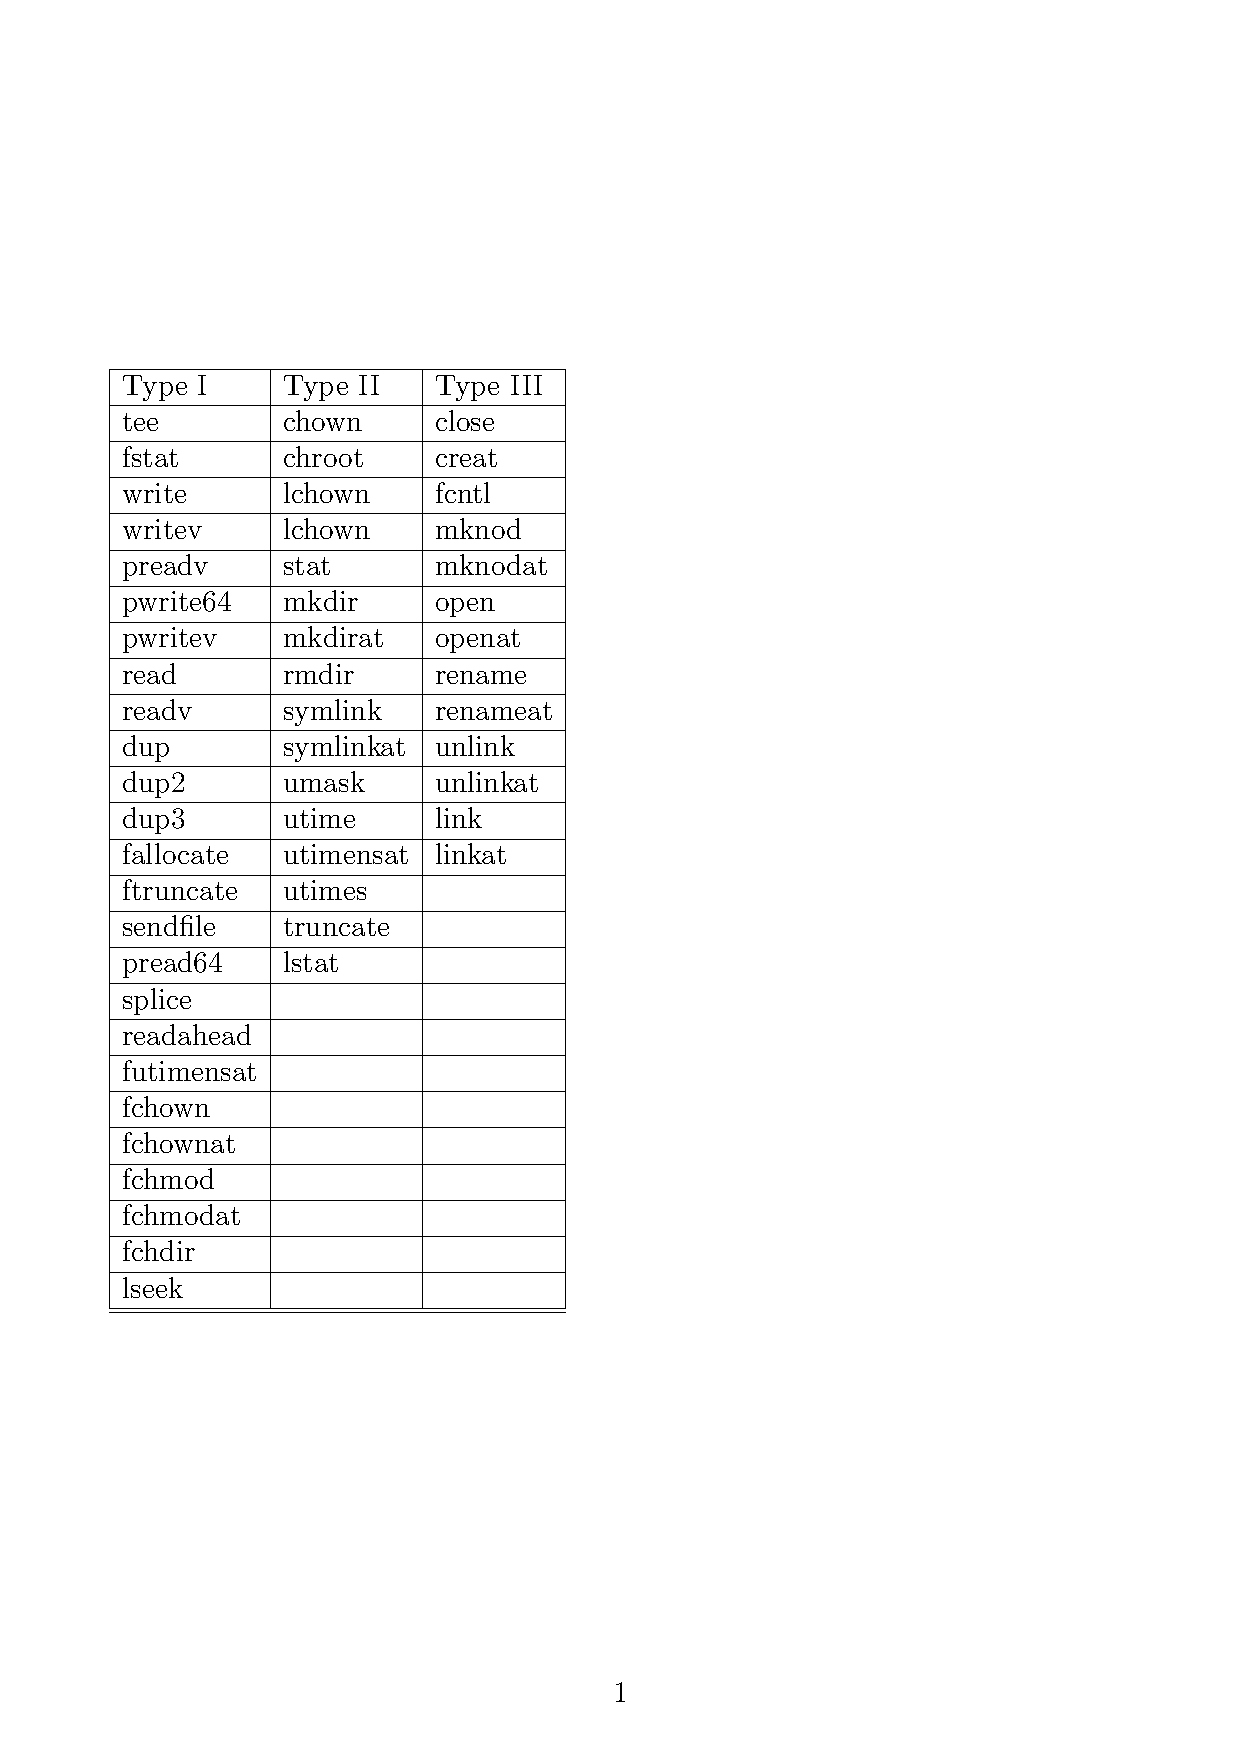
\includegraphics[width=1.0\columnwidth]{SysCalls}
  \caption{System call types}
  \label{fig:syscalltypes}
\end{figure}

We have identified a set of system calls that have to be mapped to PVM semantics.
These system calls belong to three types, as shown in ~\ref{fig:syscalltypes}

Type I, system calls that no not cause nodes in the graph to version.

Type II, system calls that act directly on paths and not via file handles.
PVM models type II system calls using the ephemeral local object $\phi$ as follows:

$$get(\phi)$$
$$get(\phi, eqv(g))$$
$$drop(\phi, eqv(g))$$
$$drop(\phi)$$

Type III, special case system calls that have to be defined individually.
Some type III system call mappis are shown below:

\texttt{Open} take a file path and returns a file descriptor.
This operation is mapped in OPUS as,

$$l = open(g):$$
$$get(l)$$
$$get(l, eqv(g))$$

\texttt{Close} takes a file descriptor as argument and releases the underlying resource.
This operation is mapped in OPUS as,

$$close(l):$$
$$drop(l, globals(l))$$
$$drop(l)$$

\texttt{Unlink} takes a file path as argument and deletes the file from the filesystem.
This is is mapped in OPUS as,

$$unlink(g):$$
$$get(\phi)$$
$$get(\phi,eqv(g))$$
$$\forall r.r \in locals(g).r \neq \phi.untie(r,g)$$
$$drop(\phi,eqv(g))$$
$$erem(eqv(g),g)$$
$$drop(\phi)$$

% TODO: Is performance evaluation sufficient?
% What about graph generation, storage etc?

\section{Performance Evaluation}
In this section we evaluate the overheads imposed by OPUS on scientific activities and workloads.
We limit our scope by focussing on the most common types of activities that a scientific user typically performs, namely, 
package installation, file editing, use of version control, code compilation, file archival/extraction and execution of scientific workloads.
Since the scientific applications can themselves be diverse, we further categorise them into compute bound, I/O bound and applications that require a runtime environment (e.g. python).
We choose representative workloads for each of these categories.

We are intersted in evaluating two aspects of our system:
\begin{enumerate}
\item Temporal overheads introduced by the provenance capture and analysis components on end user applications.
\item Spatial overheads (memory and disk space) of processing and storing provenance data.
\end{enumerate}

To evaluate the temporal overheads we first setup a baseline for each type of activity by running the representative application for that type with OPUS disabled.
We then enable OPUS and run the same set of applications in the OPUS enabled environment.

OPUS has a number of configuration options for both the frontend and backend.
The frontend can be configured to run in two modes:
\begin{enumerate}
\item Full capture, where all events for which interposition is available are captured.
\item Lite capture, where certain events (e.g. reads and writes) are discarded.
\end{enumerate}

Similarly, the backend analyser can be configured to run in,
\begin{enumerate}
\item Logging mode, where the analyser does minimum processing on the system call data and logs it to disk.
\item PVM mode, where PVM operations are applied on each event received and a DAG is constructed.
\end{enumerate}

We evaluate OPUS with various configuration options for both the frontend and backend.
Each experiment is repeated ten times to account for variances in runtime due to system effects that we do not control.

% 
% We measure the overheads under various configurations for both the OPUS frontend and backend.
% i.e. full-fat and lite modes, backend in logging mode and PVM mode.
% Use of embedded vs standalone database.

% Application list:
% Code Compilation: Kernel Compile. Compilation of CBLAS, LAPACK, FFTW, LAPACK++.
% Package Installation: Use of apt-get and pip to install packages.
% Version Control: Git.
% File I/O: Postmark
% Archiving/Extracting: tar and untar
% Application Execution: BioPerl and BioPython, BLAST

% Discussion on what is the cause of the overheads on each of these workloads.
% Too many file matadata updates?
% Too many process and thread creations?
% Low overheads coz its CPU intensive? What meaningful provenance is recorded?
% Effect of analysis running on the same machine?
% Categorize syscalls. Which get called a lot, for what type of workload.
% Time breakdown by syscall.

% NOTES: How was PASS, CDE, Burrito evaluated?
% PASS and PA-NFS: linux compile, Postmark, Mercurial, BLAST
% CDE:
% BURRITO: 


\begin{itemize}
\item Temporal overheads of using OPUS. (Interposition overheads)
\item Pathological case, \texttt{man} command. Single char reads and writes. (should this be in implementation?)
\item Optimisations performed, aggregation, OPUS Lite etc. (implementation?)
\item Performance evaluation of the analyser backend. Cost of DB operations.
\item Spatial overheads: Average space used to store provenance, for scientific workloads.
\item Comparing Neo4J with SQLite?
\item https://docs.google.com/spreadsheets/d/13QqrShPEgjC91RKLnzcIfuliM-mZovhjO2vRkewWyJ0/edit?usp=sharing
\item Look at how CDE was evaluated. SPEC, Real-World benchmarks.
\end{itemize}

\section{Tools for Scientific Workloads}
\begin{itemize}
\item Debugging context changes. Detect changes in environment, command line params, library versions linked etc.
\item Show the command and output snapshot.
\item Tracking Computations. Capture scientific workflow from ad-hoc steps. Tools to visualise and scriptise the workflow.
\item Show the provenance graph figure here.
\item Archiving for compliance. EPSRC mandate to provide code and data used to produce results. Workflow archive tool, enables scientists to archive and upload their code and data used in experiments.
\item Post-hoc workflow construction
% NOTE: Maybe merge workflow tracking and archiving into one tool?
\end{itemize}

% TODO: Secure provenance?

\section{Beyond Scientific Computing}
\begin{itemize}
\item OPUS as a provenance system can be used beyond the use-case of scientific computing.
\item The OPUS backend can consume data from any system call level tracing producer.
\item We have ported OPUS to work with data generated from DTrace instrumentation on FreeBSD.
\item This is in the context of the CADETS project. Explain CADETS briefly here.
\item OPUS will be one of the consumers of CADETS trace data and will generate provenance graph.
\item OPUS will run on the network and store data for higher level analysis.
\item In the context of CADETS what assurances can a system like OPUS provide about the data it stores to disk.
\item Can an attacker compromise the machine on which OPUS is running on and modify or corrupt the data?
\end{itemize}


\chapter{Non-Repudiable, Assertable Disk I/O} % NORAD
\section{Motivation}
\begin{itemize}
\item Previous chapter looked at adding provenance support for scientific data and computational pipelines. 
\item However, provenance capture is not limited to the use in scientific computing alone. The use of provenance in systems security is gaining more and more importance.
\item The goal of the CADETS project is to enable provenance support for the detection and if possible prevention of security attacks in systems.
\item The CADETS project is looking at OPUS as a potential system that generates provenance from raw event traces generated on such systems.
\item When used in such a security context, OPUS needs to provide certain guarantees about the authenticity and integrity of provenance it is generating and storing on disk.
\item Currently, OPUS has a large TCB. A significant part of this TCB is the underlying OS.
\item If the OS gets compromised can one still reason about the trustworthiness of provenance that OPUS generates?

\item There is now commerically available hardware support for isolated execution, see SGX section.
\item Executing OPUS on SGX will ensure that critical bits in OPUS memory are protected and the provenance graph generated by OPUS is trustworthy.
\item However, to store this provenance OPUS still needs to call into the underlying OS.
\item  % TODO: from here....

\item However, the achilles heel in such a system is reasoning about the trustworthiness and integrity of data.
\item Integrity has previously been solved using crypto techniques, hashing, checksumming, encryption etc.
\item Onus on the application to use these techniques. However, this still not sufficient.
\item Applications must trust the underlying OS to faithfully perform their I/O.
\item OSes get routinely compromised and this questions the trustworthiness of data and its provenance.
\item In this chapter we set out to solve the issue of trustworthiness of data for the purposes of asserting and correlating control-flow provenance collected with the data on the system.
\item Can we do this with the OS out of the trust boundary?
\end{itemize}

\section{Trusted Execution of applications on Untrusted OSes}
\begin{itemize}
\item Talk about InkTag, Sego etc.
\item SGX, hardware assisted inverse sandbox for the secure execution of applications on untrusted system software.
\end{itemize}

% TODO: What is SGX, how does it work?

\section{NORAD}
\begin{itemize}
\item Threat Model and TCB.
\item Use of SGX for trusted execution of applications.
\item How data provenance is captured from application to device.
\item APSYS'17 paper.
\end{itemize}

\subsection{Prototype}
\begin{itemize}
\item Library to perform raw block reads and writes.
\item Emulation of firmware on a stackable block device driver.
\end{itemize}

\subsection{Evaluation}
\begin{itemize}
\item Latency and Throughput compared to \texttt{dd} performing direct I/O.
\item Use of different block sizes.
\item compare use of cmac vs vmac.
\item Use of hotcalls to avoid context switching.
\end{itemize}

\chapter{Future Directions and Conclusions}
\begin{itemize}
\item Integration with a real-world filesystem.
\item User of smart devices to verify OS actions.
\item Approaches:
(i) Execute enclave code within the kernel.
(ii) Use of a block based FUSE file system implementation.
(iii) Use of smart SSDs and USBs to verify OS requests.
\item Extend design to other forms of I/O, specifically network I/O.

\item Conclusions: 
(i) Shown that its possible to build systems for control-flow provenance and data-flow provenance.
(ii) Building blocks for provenance as a first class construct.
\end{itemize}




%%%%%%%%%%%%%%%%%%%%%%%%%%%%%%%%%%%%%%%%%%%%%%%%%%%%%%%%%%%%%%%%%%%%%%%%%%%%%%%%
%% Bibliography:
%%
\cleardoublepage
\phantomsection
\addcontentsline{toc}{chapter}{Bibliography}
\bibliographystyle{plainnat}
\bibliography{thesis}



%%%%%%%%%%%%%%%%%%%%%%%%%%%%%%%%%%%%%%%%%%%%%%%%%%%%%%%%%%%%%%%%%%%%%%%%%%%%%%%%
%% Appendix:
%%

\appendix

\chapter{Extra Information}
Some more text ...



%%%%%%%%%%%%%%%%%%%%%%%%%%%%%%%%%%%%%%%%%%%%%%%%%%%%%%%%%%%%%%%%%%%%%%%%%%%%%%%%
%% Index:
%%
\printthesisindex

\end{document}
